\subsection{Ejercicio 11}
\graphicspath{ {img/11} }

Comprobar la firma criptográfica de un paquete es realmente sencillo una vez que utilizamos \texttt{gpg} en los apartados anteriores. Lo primero es importar la clave pública del desarrollador, que como indica la propia web de \href{https://keepassxc.org/}{KeePassXC}, se puede descargar desde el keyserver \url{openpgp.org} con el comando

\begin{minted}[
    frame=single,
    framesep=8pt,
    breaklines,
    bgcolor=bgGray
]{bash}
    gpg --keyserver keys.openpgp.org --recv-keys BF5A669F2272CF4324C1FDA8CFB4C2166397D0D2
\end{minted}

Una vez descargado, podemos comprobar la firma del archivo con el comando

\begin{minted}[
    frame=single,
    framesep=8pt,
    breaklines,
    bgcolor=bgGray
]{bash}
    gpg --verify gpg --verify KeePassXC-2.7.10-x86_64.AppImage.sig
\end{minted}

de la misma forma que hacíamos con los correos electrónicos.

\begin{figure}[H]
    \centering
    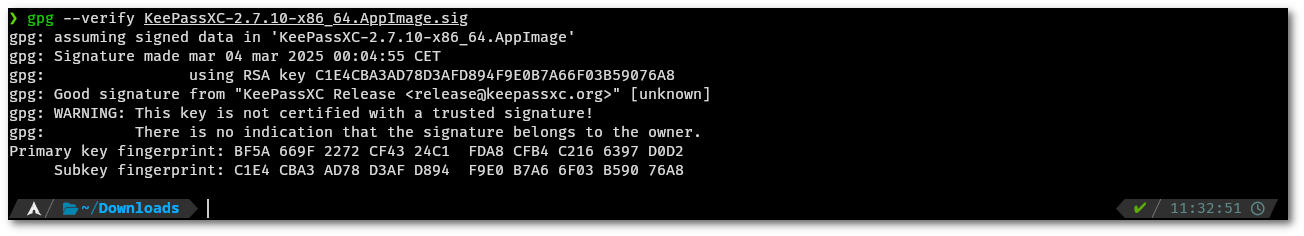
\includegraphics[width=\textwidth]{keepassxc-signature.png}
    \caption{Comprobación de la firma con \texttt{gpg}}
\end{figure}

Sí, podemos asegurar que tenemos la clave pública adecuada una firma criptográfica es una manera mucho más segura de verificar que no se modificó el paquete, ya que el hash es una buena forma de comprobar la integridad que sería muy fácil de evadir en caso de querer servir un paquete comprometido, simplemente tendríamos que mostrar el hash correspondiente al paquete malicioso en la web. Con la firma esto es imposible si ya tenemos descargada la clave pública del desarrollador.

Tanto es así que los gestores de paquetes en GNU/Linux utilizan el método de la firma para verificar la integridad y la seguridad de los paquetes, ya que en esta situación, los paquetes se pueden descargar de diversos repositorios, llamados espejos que podrían gestionar diferentes personas o entidades. Así, todos los paquetes están firmados por el mantenedor de la distribución que estemos utilizando, asegurando que no se modificaron los paquetes independientemente del espejo que utilicemos, siempre que se valide la firma con la clave pública del mantenedor.